\chapter{Conception et Architecture du Système}
\label{chap:system_design_architecture}

\section{Introduction}

\par Après avoir examiné les exigences fonctionnelles et non fonctionnelles de \textbf{TuniPark}, cette étape consiste à définir l'architecture du système ainsi que les choix techniques retenus pour son développement. L'objectif est de concevoir une architecture modulaire, évolutive et facilement maintenable, capable de répondre aux différents besoins de l'application.

\par Ce chapitre présente tout d'abord l'architecture générale du système, puis décrit les architectures logique et physique. Les principales technologies utilisées sont ensuite présentées avant d'introduire la conception de la base de données ainsi que les principaux diagrammes UML réalisés durant la phase de conception.
\section{Architecture du système}

\par L'application \textbf{TuniPark} repose sur une architecture client--serveur composée d'une application mobile destinée aux utilisateurs, d'une interface web réservée à l'administrateur, d'un serveur Backend, d'un microservice d'IA ainsi que d'une base de données relationnelle. Cette architecture assure une séparation claire entre les différentes couches du système afin d'améliorer la maintenabilité, la sécurité et l'évolutivité de l'application.

    \subsection{Architecture logique}

    \par Cette partie décrit les principaux composants logiciels de l'application ainsi que leurs interactions. Le système est organisé en cinq couches : la couche de présentation, la couche métier, la couche d'accès aux données, la couche de données et la couche des services externes.

\par La couche de présentation comprend l'application mobile développée avec \textbf{Flutter} \cite{flutter}, destinée aux utilisateurs, ainsi que l'interface web d'administration développée avec \textbf{Angular} \cite{angular}. L'application mobile permet notamment de rechercher des parkings, gérer des sessions de stationnement, publier des parkings privés, effectuer des paiements, consulter les statistiques personnelles et recevoir des notifications. L'interface web permet à l'administrateur de superviser les utilisateurs, les parkings, les paiements et les différentes informations de la plateforme.

\par La couche métier est implémentée à l'aide du framework \textbf{NestJS} \cite{nestjs}. Elle expose une API REST sécurisée et regroupe l'ensemble de la logique métier de l'application. Cette couche est composée de plusieurs modules, notamment l'authentification, la gestion des utilisateurs, des parkings, des sessions de stationnement, des parkings privés, des paiements, des notifications, des statistiques ainsi que du système de recommandation basé sur l'IA.

\par La couche d'accès aux données repose sur \textbf{Prisma ORM} \cite{prisma}. Celui-ci facilite les échanges entre le Backend et la base de données PostgreSQL tout en garantissant une manipulation fiable et sécurisée des données.

\par La couche de données fait appel à une base de données de type relationnel \textbf{PostgreSQL} \cite{postgresql}. Elle assure le stockage des informations relatives aux utilisateurs, aux parkings, aux sessions de stationnement, aux paiements, aux notifications ainsi qu'aux interactions exploitées par le système de recommandation.

\par Enfin, l'application s'appuie sur plusieurs services externes. Les images des parkings sont stockées sur \textbf{Cloudinary} \cite{cloudinary}, les notifications Push sont envoyées grâce à \textbf{Firebase Cloud Messaging (FCM)} \cite{firebase}, les paiements électroniques sont réalisés via \textbf{Flouci} \cite{flouci}, les courriers électroniques sont envoyés à l'aide de \textbf{Nodemailer} \cite{nodemailer}, tandis que l'envoi des codes OTP par SMS est prévu via \textbf{Twilio} \cite{twilio}. Un microservice développé avec \textbf{FastAPI} \cite{fastapi} héberge également le modèle d'IA basé sur l'algorithme \textbf{Random Forest} \cite{breiman2001randomforest}, chargé de calculer les recommandations de parkings.

\begin{figure}[H]
    \centering
    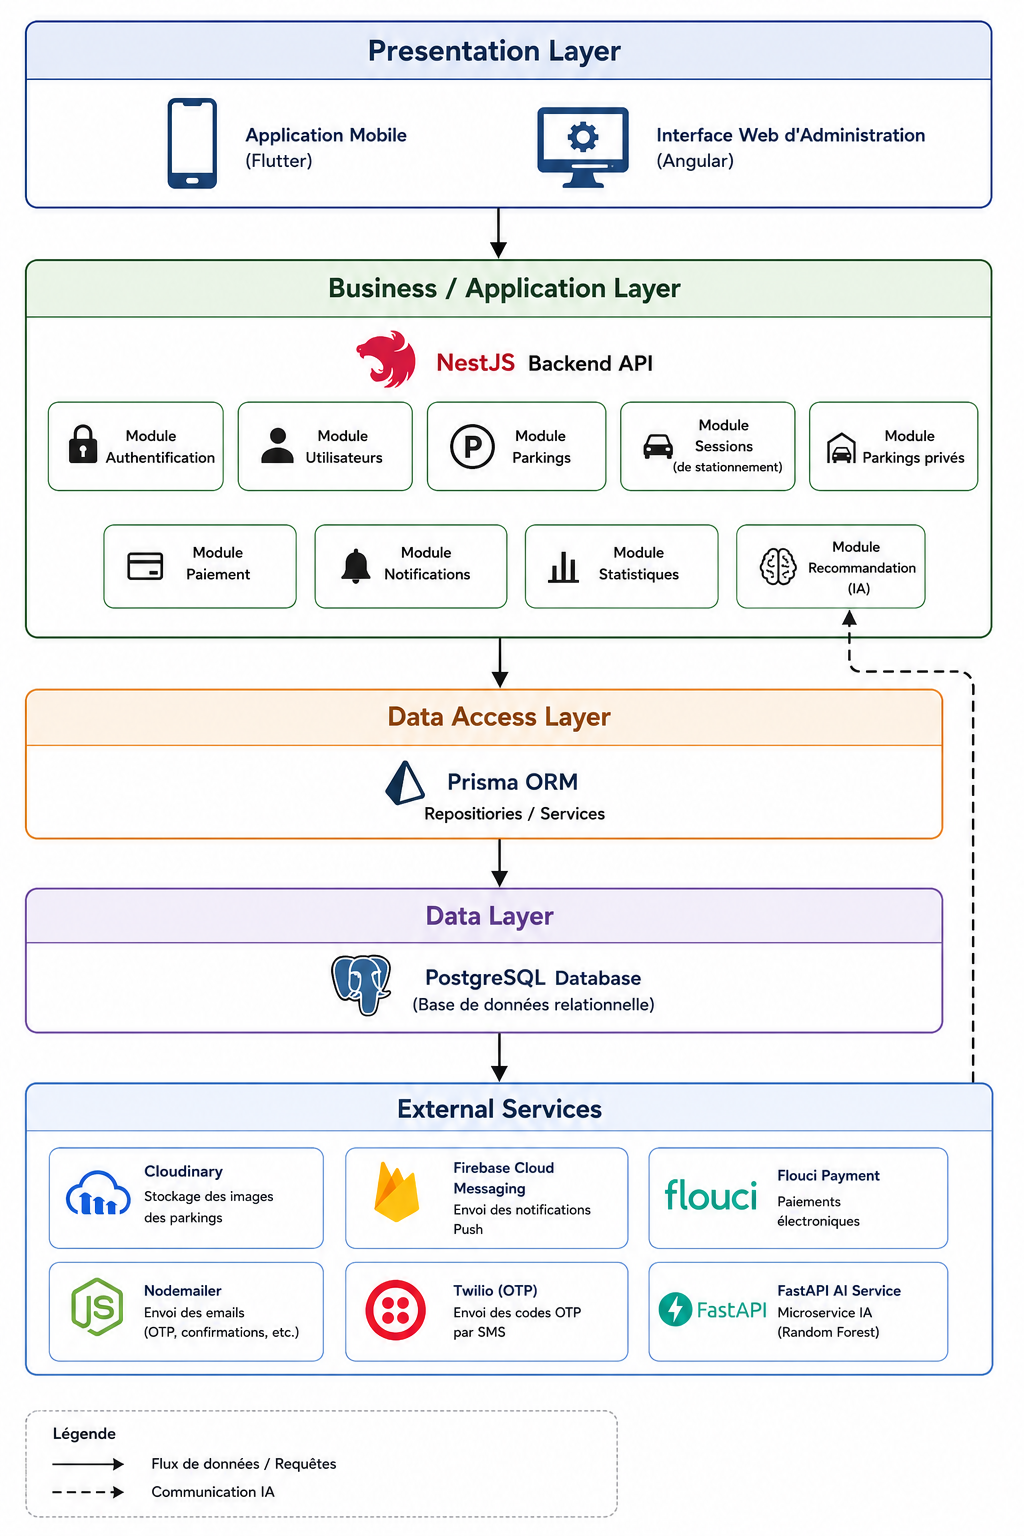
\includegraphics[width=0.60\textwidth]{img/architecturelogi.png}
    \caption{Architecture logique de TuniPark}
    \label{fig:logical_architecture}
\end{figure}

\par Comme l'illustre la Figure~\ref{fig:logical_architecture}, les interfaces mobile et web communiquent avec le Backend via des requêtes REST sécurisées. Le Backend centralise la logique métier, interagit avec PostgreSQL par l'intermédiaire de Prisma ORM et communique avec les différents services externes tels que Cloudinary, Flouci, Firebase Cloud Messaging, Nodemailer ainsi que le microservice d'IA développé avec FastAPI.
\subsection{Architecture physique}

\par Cette architecture présente le déploiement réel des différents composants de l'application TuniPark. Le système est accessible à travers deux interfaces clientes : l'application mobile développée avec \textbf{Flutter} et l'interface web d'administration développée avec \textbf{Angular}.

\par L'interface web d'administration est hébergée sur \textbf{Vercel} \cite{vercel}, tandis que le Backend développé avec \textbf{NestJS}, le microservice d'IA développé avec \textbf{FastAPI} ainsi que la base de données \textbf{PostgreSQL} sont déployés sur \textbf{Render} \cite{render}. Les interfaces clientes communiquent avec le Backend au moyen de requêtes HTTPS vers une API REST sécurisée.

\par Le Backend centralise la logique métier de l'application et assure la communication avec la base de données ainsi qu'avec les différents services externes. Les images des parkings sont stockées sur \textbf{Cloudinary}, les notifications Push sont envoyées via \textbf{Firebase Cloud Messaging}, les paiements électroniques sont traités par \textbf{Flouci} et les courriers électroniques sont envoyés à l'aide de \textbf{Nodemailer}.

\par Le service \textbf{Twilio} est prévu pour l'envoi des codes OTP par SMS, mais il n'est pas encore opérationnel dans la version actuelle de l'application. Le microservice FastAPI héberge le modèle de recommandation basé sur l'algorithme Random Forest et communique avec le Backend NestJS à travers des requêtes HTTP.

\begin{figure}[H]
    \centering
    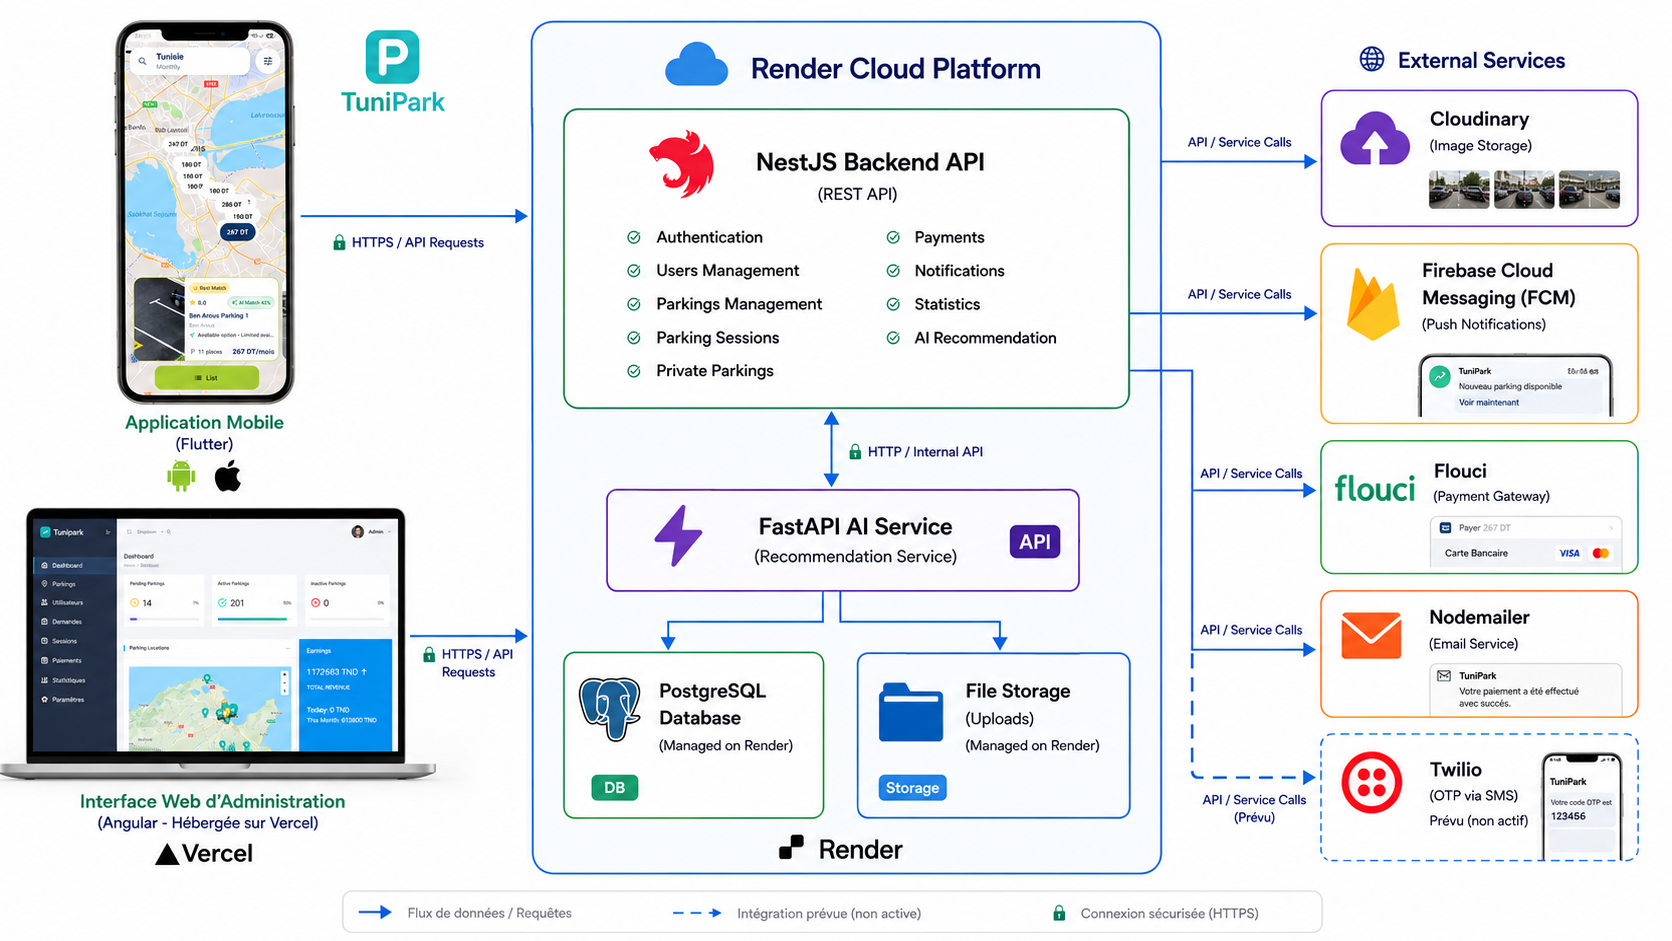
\includegraphics[width=0.95\textwidth]{img/physique.png}
    \caption{Architecture physique de l'application TuniPark}
    \label{fig:physical_architecture}
\end{figure}

\par Comme le montre la Figure~\ref{fig:physical_architecture}, les différents composants sont déployés sur des services Cloud distincts. Cette séparation permet de simplifier le déploiement, de faciliter la maintenance et de faire évoluer indépendamment le Backend, l'interface web et le service d'IA.
\section{Choix techniques}

\par Les technologies retenues pour le développement de l'application \textbf{TuniPark} ont été sélectionnées en fonction des exigences du projet, notamment en matière de performance, de sécurité, de maintenabilité et d'évolutivité. L'objectif était de mettre en place une architecture moderne, reposant sur des outils fiables, afin de concevoir une application mobile, une interface web d'administration, un Backend sécurisé et une base de données performante, tout en assurant l'interfaçage avec des services externes et un système de recommandation basé sur l'IA.\subsection{Flutter}

\par Flutter \cite{flutter} a été choisi pour développer l'application mobile de TuniPark. Ce framework développé par Google permet de concevoir une application multiplateforme à partir d'une seule base de code, compatible avec Android et iOS.

\par L'application mobile permet aux utilisateurs de rechercher des parkings, consulter leur disponibilité sur une carte interactive, démarrer et arrêter une session de stationnement, effectuer des paiements, gérer leurs parkings privés ainsi que recevoir des notifications en temps réel.

\begin{figure}[H]
    \centering
    
\includegraphics[width=0.12\textwidth]{img/flutter_logo.png}
    \caption{Logo du framework Flutter}
\end{figure}

\subsection{Angular}

\par Angular \cite{angular} a été utilisé pour développer l'interface web d'administration de TuniPark. Cette application permet à l'administrateur de superviser la plateforme, gérer les utilisateurs, valider les demandes de parkings privés, consulter les statistiques ainsi que suivre l'ensemble des opérations réalisées sur le système.

\par L'application Angular communique avec le Backend via des API REST sécurisées.

\begin{figure}[H]
    \centering
    
\includegraphics[width=0.15\textwidth]{img/angular.png}
    \caption{Logo du framework Angular}
\end{figure}

\subsection{NestJS}

\par Le Backend de TuniPark a été développé avec NestJS \cite{nestjs}. Ce framework basé sur Node.js et TypeScript offre une architecture modulaire facilitant l'organisation des différents modules de l'application.

\par Il centralise la logique métier du système, notamment l'authentification, la gestion des utilisateurs, des parkings, des sessions de stationnement, des paiements, des notifications, ainsi que la communication avec le microservice d'IA.

\begin{figure}[H]
    \centering
    
\includegraphics[width=0.22\textwidth]{img/nestjs_logo.png}
    \caption{Logo du framework NestJS}
\end{figure}

\subsection{PostgreSQL et Prisma}

\par Les données de TuniPark sont stockées dans une base de données relationnelle PostgreSQL \cite{postgresql}. Cette solution garantit l'intégrité des données, une gestion fiable des liens entre les entités, ainsi que de bonnes performances lors des requêtes.
\par L'accès à la base de données est assuré par Prisma ORM \cite{prisma}, qui simplifie les opérations de création, de lecture, de modification et de suppression des données tout en offrant une sécurité de typage grâce à TypeScript.

\begin{figure}[H]
   \centering
   
\includegraphics[width=0.16\textwidth]{img/postgresql_logo.png}
    \caption{Logo de PostgreSQL}
\end{figure}


\subsection{FastAPI et Random Forest}

\par Pour offrir une meilleure expérience aux utilisateurs, TuniPark intègre un microservice d'IA développé avec FastAPI \cite{fastapi} en Python. Ce service expose des API REST consommées par le Backend NestJS.

\par Le modèle de recommandation repose sur l'algorithme Random Forest \cite{breiman2001randomforest}. Il analyse plusieurs critères tels que la distance entre l'utilisateur et le parking, le taux de disponibilité, le taux de conversion des consultations en réservations, le taux de prolongation des sessions ainsi que le tarif du parking afin de calculer un score de recommandation.

\par Les parkings sont ensuite classés selon ce score afin de proposer en priorité les emplacements les plus pertinents pour chaque utilisateur.

\begin{figure}[H]
    \centering
    
\includegraphics[width=0.15\textwidth]{img/python_logo.png}
    \caption{Microservice IA développé avec FastAPI}
\end{figure}

\subsection{Authentification JWT}

\par La sécurisation des accès repose sur JSON Web Token (JWT) \cite{jwt}. Après une authentification réussie, le Backend génère un Access Token valide pendant une heure ainsi qu'un Refresh Token valide pendant trois jours.

\par Lorsque l'Access Token expire, un intercepteur Dio renouvelle automatiquement celui-ci à l'aide du Refresh Token sans intervention de l'utilisateur. Si le Refresh Token arrive également à expiration, la session est automatiquement fermée, les informations locales sont supprimées et l'utilisateur est orienté vers la page de connexion.

\begin{figure}[H]
    \centering
    
\includegraphics[width=0.10\textwidth]{img/jwt_logo.png}
    \caption{Authentification basée sur JWT}
\end{figure}

\subsection{Cloudinary}

\par Cloudinary \cite{cloudinary} est utilisé pour le stockage des images des parkings. Ce service Cloud permet d'héberger les images, de les optimiser automatiquement et de fournir des liens sécurisés pour leur affichage dans l'application.

\begin{figure}[H]
    \centering
    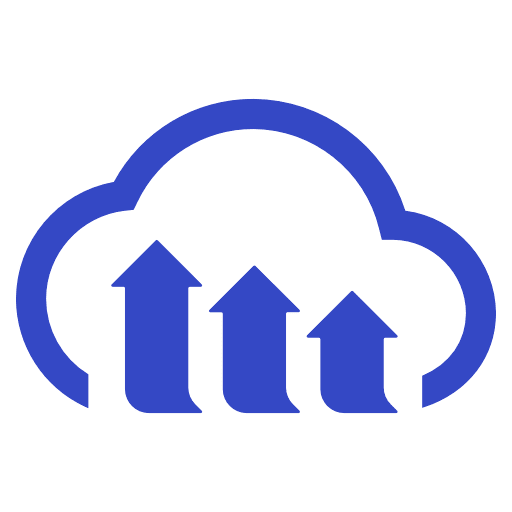
\includegraphics[width=0.18\textwidth]{img/cloudinary_logo.png}
    \caption{Logo de Cloudinary}
    \label{fig:cloudinary_logo}
\end{figure}

\subsection{Firebase Cloud Messaging}

\par Firebase Cloud Messaging (FCM) \cite{firebase} permet l'envoi de notifications Push aux utilisateurs. Il est utilisé pour informer les utilisateurs des validations de leurs parkings, des paiements, des rappels de session ainsi que des différentes notifications générées par l'application.
\begin{figure}[H]
    \centering
    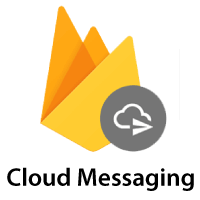
\includegraphics[width=0.18\textwidth]{img/firebase_logo.png}
    \caption{Logo de Firebase Cloud Messaging}
    \label{fig:fcm_logo}
\end{figure}



\subsection{Flouci}

\par Flouci \cite{flouci} est la solution de paiement électronique intégrée à TuniPark. Elle permet aux utilisateurs d'effectuer leurs paiements de manière sécurisée directement depuis l'application mobile avant le démarrage d'une session de stationnement.

\begin{figure}[H]
    \centering
    
\includegraphics[width=0.18\textwidth]{img/flouci_logo.png}
    \caption{Logo de Flouci}
    \label{fig:flouci_logo}
\end{figure}


\subsection{Nodemailer}

\par Nodemailer \cite{nodemailer} est utilisé pour l'envoi automatique des courriers électroniques, notamment lors de la création d'un compte, de la changement de mot de passe et de l'envoi des codes OTP par courrier électronique.

\begin{figure}[H]
    \centering
    
\includegraphics[width=0.18\textwidth]{img/nodemailer_logo.png}
    \caption{Logo de Nodemailer}
    \label{fig:nodemailer_logo}
\end{figure}


\section{Conception de la base de données}

\par La base de données de l'application \textbf{TuniPark} repose sur le SGBD relationnelles \textbf{PostgreSQL} \cite{postgresql}. Elle est structurée autour de plusieurs tables correspondant aux principaux domaines fonctionnels de l'application, notamment la gestion des utilisateurs, des parkings, des sessions de stationnement, des paiements, des notifications et des interactions utilisées par le système de recommandation.

\par L'accès aux données est assuré par \textbf{Prisma ORM} \cite{prisma}, qui facilite la définition des relations entre les entités et les opérations réalisées depuis le Backend NestJS. Cette organisation permet de préserver la cohérence des données et de faciliter l'évolution du système.

\subsection{Tables de gestion des utilisateurs et des accès}

\begin{table}[H]
\centering
\small
\renewcommand{\arraystretch}{1.25}
\begin{tabular}{|p{0.28\textwidth}|p{0.62\textwidth}|}
\hline
\textbf{Table} & \textbf{Rôle dans l'application} \\
\hline
\texttt{User} & Sauvegarde les informations des utilisateurs, notamment leur identité, leurs coordonnées, leur mot de passe, leur rôle ainsi que l'état de vérification de leur adresse électronique et de leur numéro de téléphone. Cette table contient également les informations temporaires nécessaires à la vérification et à la changement de mot de passe par code OTP. \\
\hline
\texttt{FcmToken} & Stocke les jetons Firebase associés aux appareils des utilisateurs afin de permettre l'envoi de notifications Push. Un utilisateur peut posséder plusieurs jetons lorsqu'il utilise plusieurs appareils. \\
\hline
\end{tabular}
\caption{Tables de gestion des utilisateurs et des accès}
\label{tab:user_access_tables}
\end{table}

\subsection{Tables de gestion des parkings}

\begin{table}[H]
\centering
\small
\renewcommand{\arraystretch}{1.25}
\begin{tabular}{|p{0.28\textwidth}|p{0.62\textwidth}|}
\hline
\textbf{Table} & \textbf{Rôle dans l'application} \\
\hline
\texttt{Parking} & Stocke les informations principales d'un parking, notamment son titre, son type, sa description, son emplacement, ses horaires d'ouverture, ses photos, ses caractéristiques, le nombre total de places et le nombre de places disponibles. Elle conserve également son statut de validation ainsi que la référence de son propriétaire. \\
\hline
\texttt{Tariff} & Stocke les informations tarifaires associées à un parking, telles que le prix par unité, par jour ou par mois, ainsi que les durées minimale et maximale autorisées. Chaque parking possède au maximum un tarif. \\
\hline
\end{tabular}
\caption{Tables de gestion des parkings}
\label{tab:parking_tables}
\end{table}

\subsection{Tables de gestion des sessions de stationnement}

\begin{table}[H]
\centering
\small
\renewcommand{\arraystretch}{1.25}
\begin{tabular}{|p{0.28\textwidth}|p{0.62\textwidth}|}
\hline
\textbf{Table} & \textbf{Rôle dans l'application} \\
\hline
\texttt{ParkingSession} & Stocke les sessions de stationnement ouvertes par les utilisateurs. Elle contient le parking sélectionné, les informations du véhicule, la date de début, la date de fin, la durée payée ainsi que le statut de la session. \\
\hline
\end{tabular}
\caption{Table de gestion des sessions de stationnement}
\label{tab:parking_session_table}
\end{table}

\subsection{Table de gestion des paiements}

\begin{table}[H]
\centering
\small
\renewcommand{\arraystretch}{1.25}
\begin{tabular}{|p{0.28\textwidth}|p{0.62\textwidth}|}
\hline
\textbf{Table} & \textbf{Rôle dans l'application} \\
\hline
\texttt{Payment} & Stocke les paiements associés aux sessions de stationnement. Elle conserve le fournisseur de paiement, le montant, le statut de la transaction, la référence retournée par le fournisseur ainsi que la date de confirmation du paiement. \\
\hline
\end{tabular}
\caption{Table de gestion des paiements}
\label{tab:payment_table}
\end{table}

\subsection{Tables de gestion des notifications}

\begin{table}[H]
\centering
\small
\renewcommand{\arraystretch}{1.25}
\begin{tabular}{|p{0.28\textwidth}|p{0.62\textwidth}|}
\hline
\textbf{Table} & \textbf{Rôle dans l'application} \\
\hline
\texttt{Notification} & Stocke les notifications destinées aux utilisateurs, notamment leur titre, leur contenu, leur type, les données complémentaires ainsi que leur état de lecture. \\
\hline
\texttt{FcmToken} & Associe chaque appareil à un jeton Firebase afin de transmettre les notifications Push au bon utilisateur. \\
\hline
\end{tabular}
\caption{Tables liées aux notifications}
\label{tab:notification_tables}
\end{table}

\subsection{Table utilisée par le système de recommandation}

\begin{table}[H]
\centering
\small
\renewcommand{\arraystretch}{1.25}
\begin{tabular}{|p{0.28\textwidth}|p{0.62\textwidth}|}
\hline
\textbf{Table} & \textbf{Rôle dans l'application} \\
\hline
\texttt{ParkingInteraction} & Enregistre les interactions réalisées par les utilisateurs avec les parkings. Les interactions prises en charge sont la consultation d'un parking, le démarrage d'une session et la prolongation d'une session. Ces données permettent de calculer les taux de conversion et de prolongation exploités par le système de recommandation. \\
\hline
\end{tabular}
\caption{Table utilisée par le système de recommandation}
\label{tab:recommendation_table}
\end{table}
























\subsection{Diagramme de classes}

\par Le schéma de classes décrit la configuration globale de l'application \textbf{TuniPark}. Il souligne les entités clés du système, leurs caractéristiques ainsi que les liens qui les unissent. Le modèle couvre notamment la gestion des utilisateurs, des parkings, des sessions de stationnement, des paiements, des notifications et des interactions utilisées par le système de recommandation.

\begin{figure}[H]
    \centering
    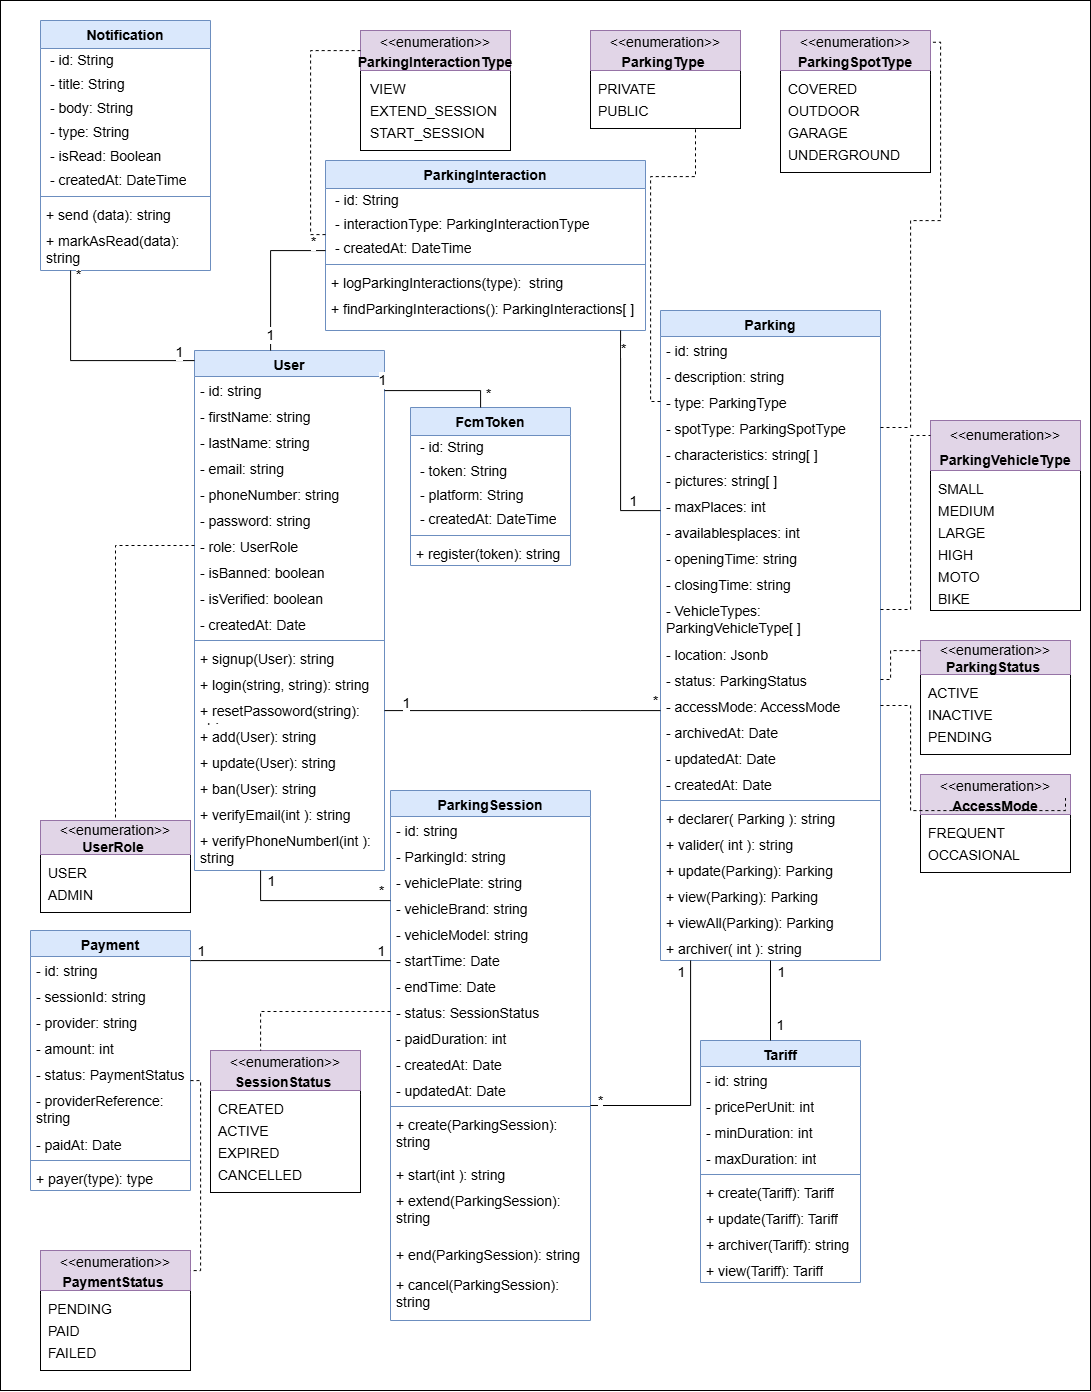
\includegraphics[width=1\textwidth]{img/class diag.drawio.png}
    \caption{Diagramme de classes de l'application TuniPark}
    \label{fig:class_diagram}
\end{figure}

\par Comme illustré dans la Figure~\ref{fig:class_diagram}, l'entité \textbf{User} occupe une place centrale dans le système. Elle contient les informations personnelles et les données nécessaires à l'authentification, ainsi que le rôle attribué à chaque utilisateur. Un utilisateur peut posséder plusieurs parkings, ouvrir plusieurs sessions de stationnement, recevoir des notifications et générer différentes interactions avec les parkings.

\par L'entité \textbf{Parking} regroupe les informations descriptives d'un espace de stationnement, notamment son type, son emplacement, ses horaires d'ouverture, ses caractéristiques, ses images, sa capacité et son statut. Chaque parking appartient à un propriétaire et peut être associé à plusieurs sessions de stationnement et interactions. Une relation individuelle relie également chaque parking à son tarif, représenté par l'entité \textbf{Tariff}.

\par L'entité \textbf{ParkingSession} représente une session de stationnement ouverte par un utilisateur dans un parking donné. Elle contient les informations du véhicule, les dates de début et de fin, la durée payée ainsi que l'état de la session. Une session peut être associée à un seul paiement, stocké dans l'entité \textbf{Payment}, qui conserve le montant, le fournisseur, le statut de la transaction et sa référence externe.

\par Les entités \textbf{Notification} et \textbf{FcmToken} prennent en charge l'envoi et le suivi des notifications. Enfin, l'entité \textbf{ParkingInteraction} enregistre les actions réalisées sur les parkings, telles que la consultation, le démarrage ou la prolongation d'une session. Ces données sont exploitées pour calculer les indicateurs utilisés par le système de recommandation.

\section{Diagrammes de séquence}

\par Les diagrammes de séquence permettent de représenter le comportement dynamique de l'application TuniPark. Ils illustrent les échanges entre les différents acteurs, l'application mobile, l'interface web d'administration, le serveur Backend, la base de données ainsi que les services externes tels que Flouci, Firebase Cloud Messaging et le microservice d'IA.

\subsection{Diagramme de séquence de l'authentification}


\par Ce diagramme met en évidence la démarche d'authentification d'un utilisateur au sein de l'application \textbf{TuniPark}. Après avoir saisi son adresse électronique ou son numéro de téléphone ainsi que son mot de passe, l'application mobile envoie une requête d'authentification au Backend. Celui-ci vérifie l'existence de l'utilisateur dans la base de données, contrôle la validité des informations d'identification puis génère un \textit{Access Token} et un \textit{Refresh Token} \cite{jwt}. Les jetons générés sont ensuite retournés à l'application et stockés de manière sécurisée sur l'appareil afin de permettre l'accès aux fonctionnalités protégées. En cas d'informations d'identification invalides, un message d'erreur est renvoyé à l'utilisateur et l'authentification est refusée.

\begin{figure}[H]
    \centering
    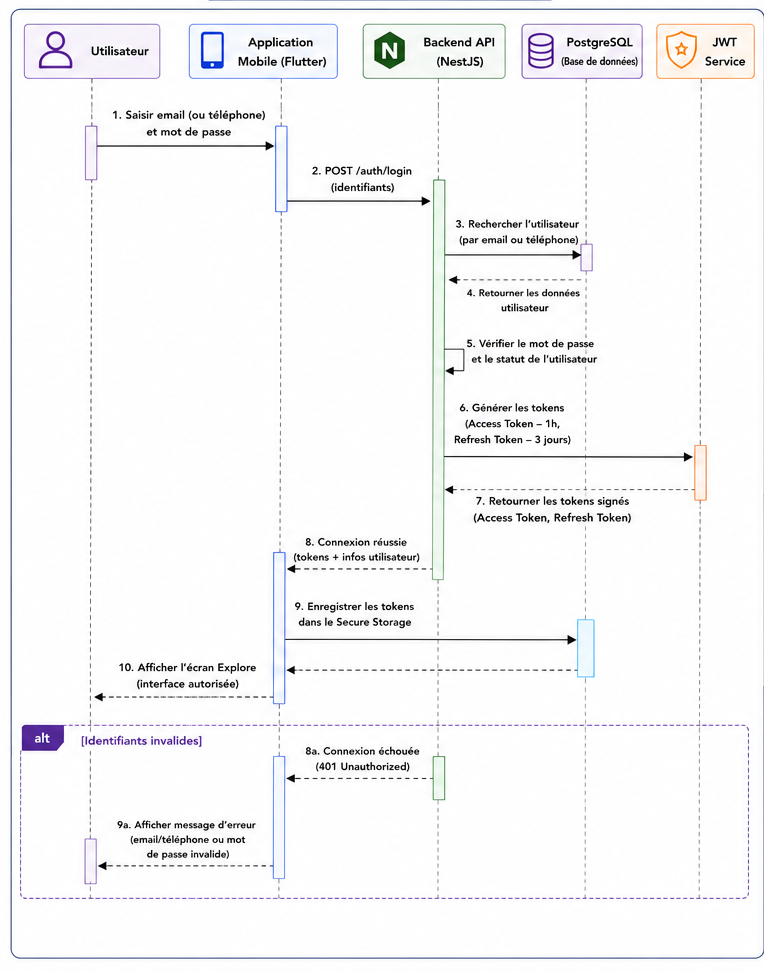
\includegraphics[width=0.95\textwidth]{img/aauth.png}
    \caption{Authentification}
    \label{fig:sequence_authentication}
\end{figure}
  
\subsection{Diagramme de séquence du renouvellement automatique du jeton}

\par Ce diagramme illustre le mécanisme de renouvellement automatique de l'\textit{Access Token}. Lorsqu'une requête retourne une réponse indiquant l'expiration du jeton d'accès, l'application utilise le \textit{Refresh Token} précédemment enregistré afin de demander un nouveau jeton au Backend. Après validation du \textit{Refresh Token}, le Backend génère un nouvel \textit{Access Token} qui est enregistré dans le stockage sécurisé de l'application. La requête initiale est ensuite relancée de manière transparente, sans intervention de l'utilisateur. Si le \textit{Refresh Token} est invalide ou expiré, les jetons sont supprimés et l'utilisateur est automatiquement redirigé vers l'écran de connexion.

\begin{figure}[H]
    \centering
    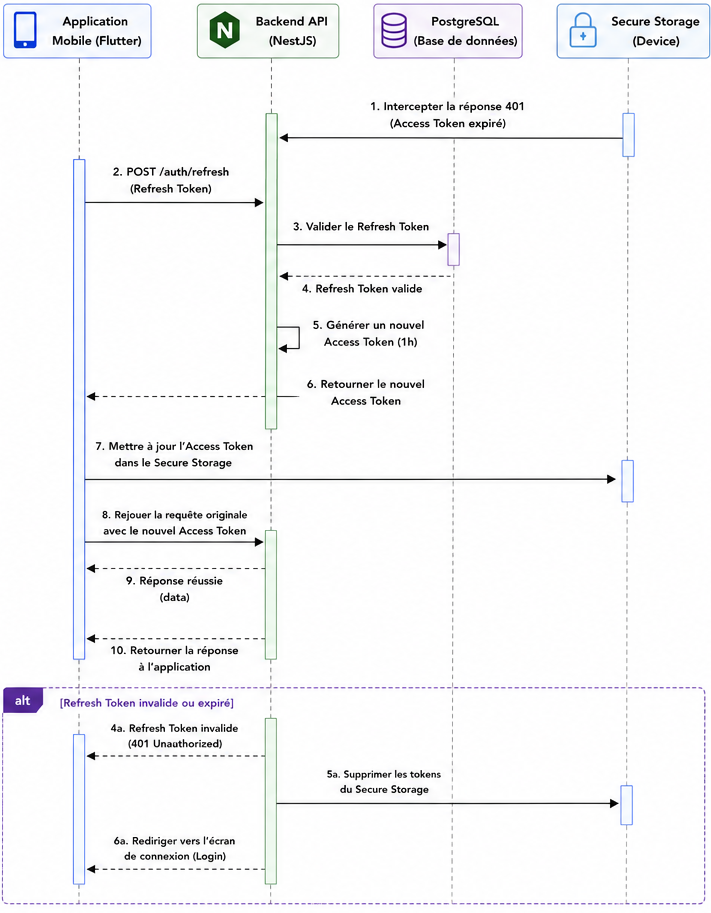
\includegraphics[width=0.7\textwidth]{img/refreshht.png}
    \caption{Renouvellement automatique du jeton}
    \label{fig:sequence_refresh_token}
\end{figure}

\subsection{Diagramme de séquence de la création d'une session de stationnement}

\par Ce diagramme illustre le processus de création d'une session de stationnement dans l'application \textbf{TuniPark}. Après avoir sélectionné un parking et renseigné les informations nécessaires, telles que la durée souhaitée, le véhicule et le numéro d'immatriculation, l'utilisateur soumet une demande de création de session. Le Backend vérifie alors la disponibilité du parking dans la base de données, crée une nouvelle session avec le statut \texttt{CREATED} et enregistre les informations correspondantes. Les détails de la session sont ensuite retournés à l'application mobile afin d'afficher un récapitulatif avant le paiement.

\begin{figure}[H]
    \centering
    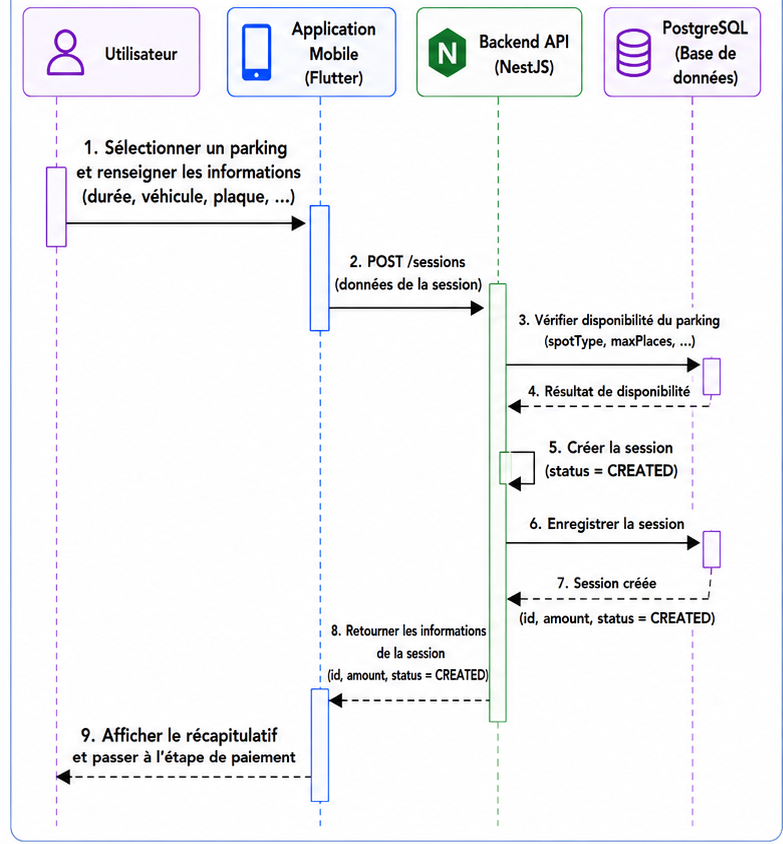
\includegraphics[width=0.65\textwidth]{img/session_creation_sequence.png}
    \caption{Création d'une session de stationnement}
    \label{fig:sequence_session_creation}
\end{figure}

\subsection{Diagramme de séquence du paiement d'une session de stationnement}

\par Ce diagramme présente le processus de paiement d'une session de stationnement à l'aide de la passerelle de paiement \textbf{Flouci} \cite{flouci}. Après validation du récapitulatif, l'utilisateur est renvoyé vers l'interface de paiement sécurisée de Flouci afin d'effectuer la transaction. Une fois le paiement terminé, Flouci transmet automatiquement le résultat au Backend via un \textit{Webhook}. En cas de succès, le Backend met à jour l'état du paiement, active la session de stationnement en changeant son statut de \texttt{CREATED} à \texttt{ACTIVE} et envoie une notification de confirmation à l'utilisateur. Si le paiement échoue ou est annulé, le paiement est marqué comme échoué, la session conserve son statut \texttt{CREATED} et l'application informe l'utilisateur afin qu'il puisse réessayer ultérieurement.

\begin{figure}[H]
    \centering
    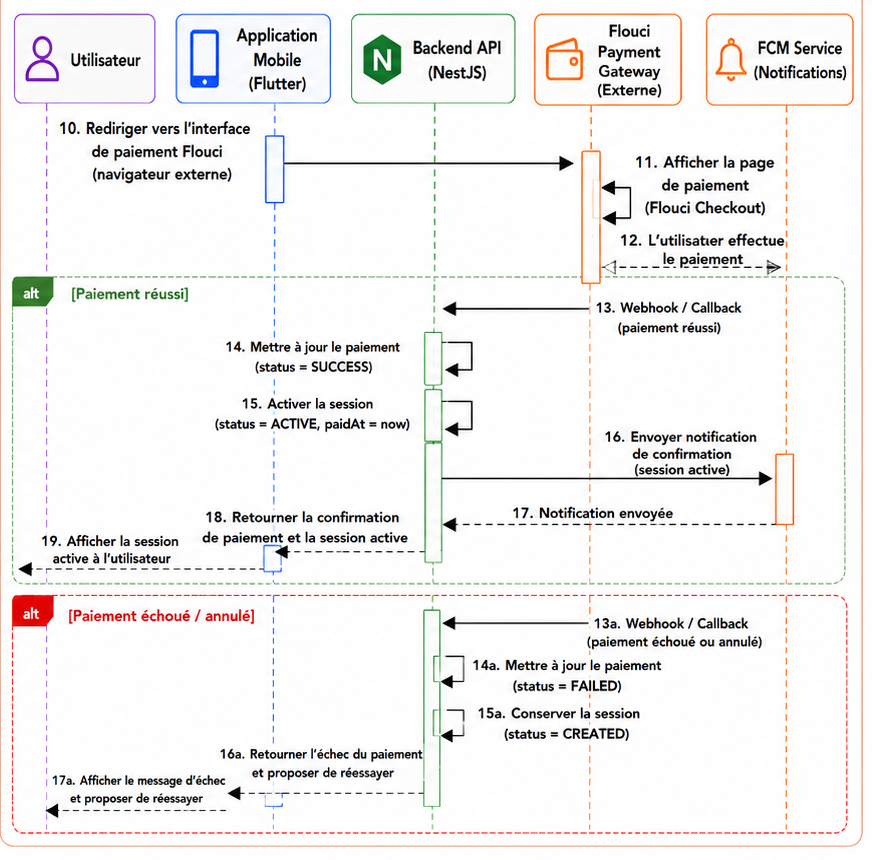
\includegraphics[width=0.85\textwidth]{img/session_payment_sequence.png}
    \caption{Paiement d'une session de stationnement}
    \label{fig:sequence_session_payment}
\end{figure}
\subsection{Diagramme de séquence de la recommandation intelligente des parkings}

\par Ce diagramme illustre le fonctionnement du système de recommandation des parkings. Après avoir obtenu la position de l'utilisateur, l'application envoie une requête au Backend. Celui-ci récupère les parkings disponibles ainsi que leurs statistiques d'utilisation, puis transmet les caractéristiques de chaque parking au microservice d'IA développé avec FastAPI \cite{fastapi}. Le modèle Random Forest \cite{breiman2001randomforest} calcule un score de recommandation pour chaque parking et retourne les résultats au Backend, qui les trie avant de les renvoyer à l'application mobile. En cas d'indisponibilité du microservice, le Backend applique automatiquement un algorithme de secours basé sur des règles afin d'assurer la continuité du service.

\begin{figure}[H]
    \centering
    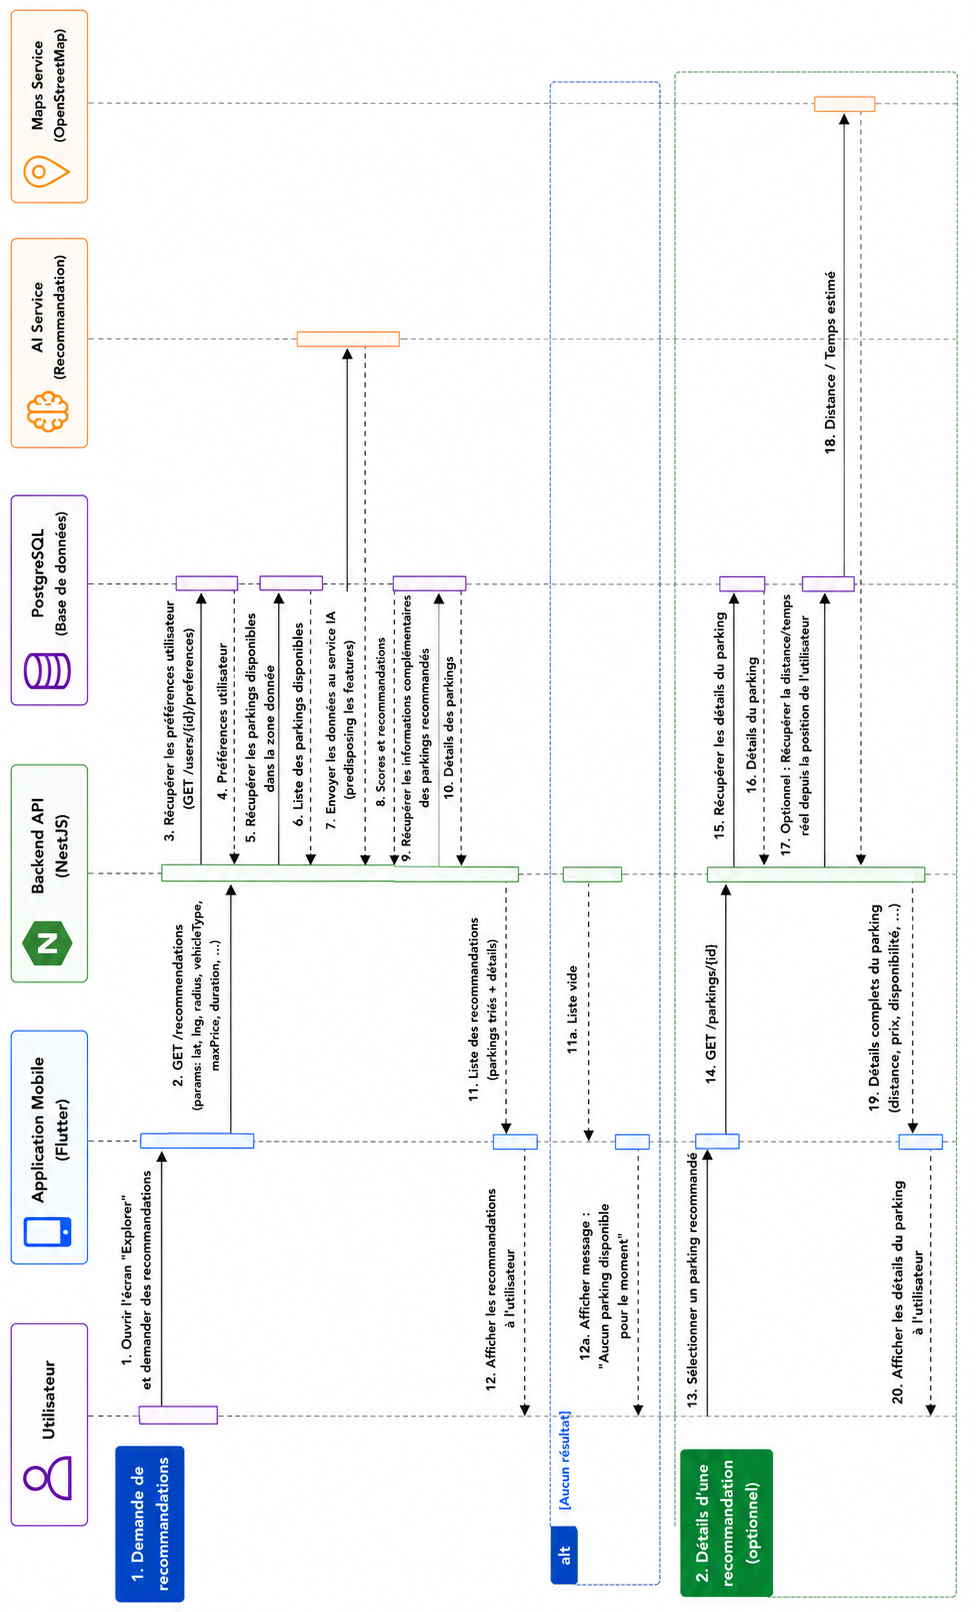
\includegraphics[width=1\textwidth]{img/ai_recom_seq.png}
    \caption{Recommandation intelligente des parkings}
    \label{fig:sequence_ai}
\end{figure}

\subsection{Diagramme de séquence de l'ajout d'un parking privé}

\par Ce diagramme présente le processus permettant à un propriétaire de proposer un parking privé sur la plateforme TuniPark. Après avoir renseigné les informations du parking et téléversé les images, l'application transmet la demande au Backend. Celui-ci vérifie les données, enregistre le parking avec le statut \textit{PENDING} puis le rend disponible dans l'interface d'administration pour validation. Après examen, l'administrateur accepte ou rejette la demande. Le propriétaire est ensuite informé de la décision par une notification.

\begin{figure}[H]
    \centering
    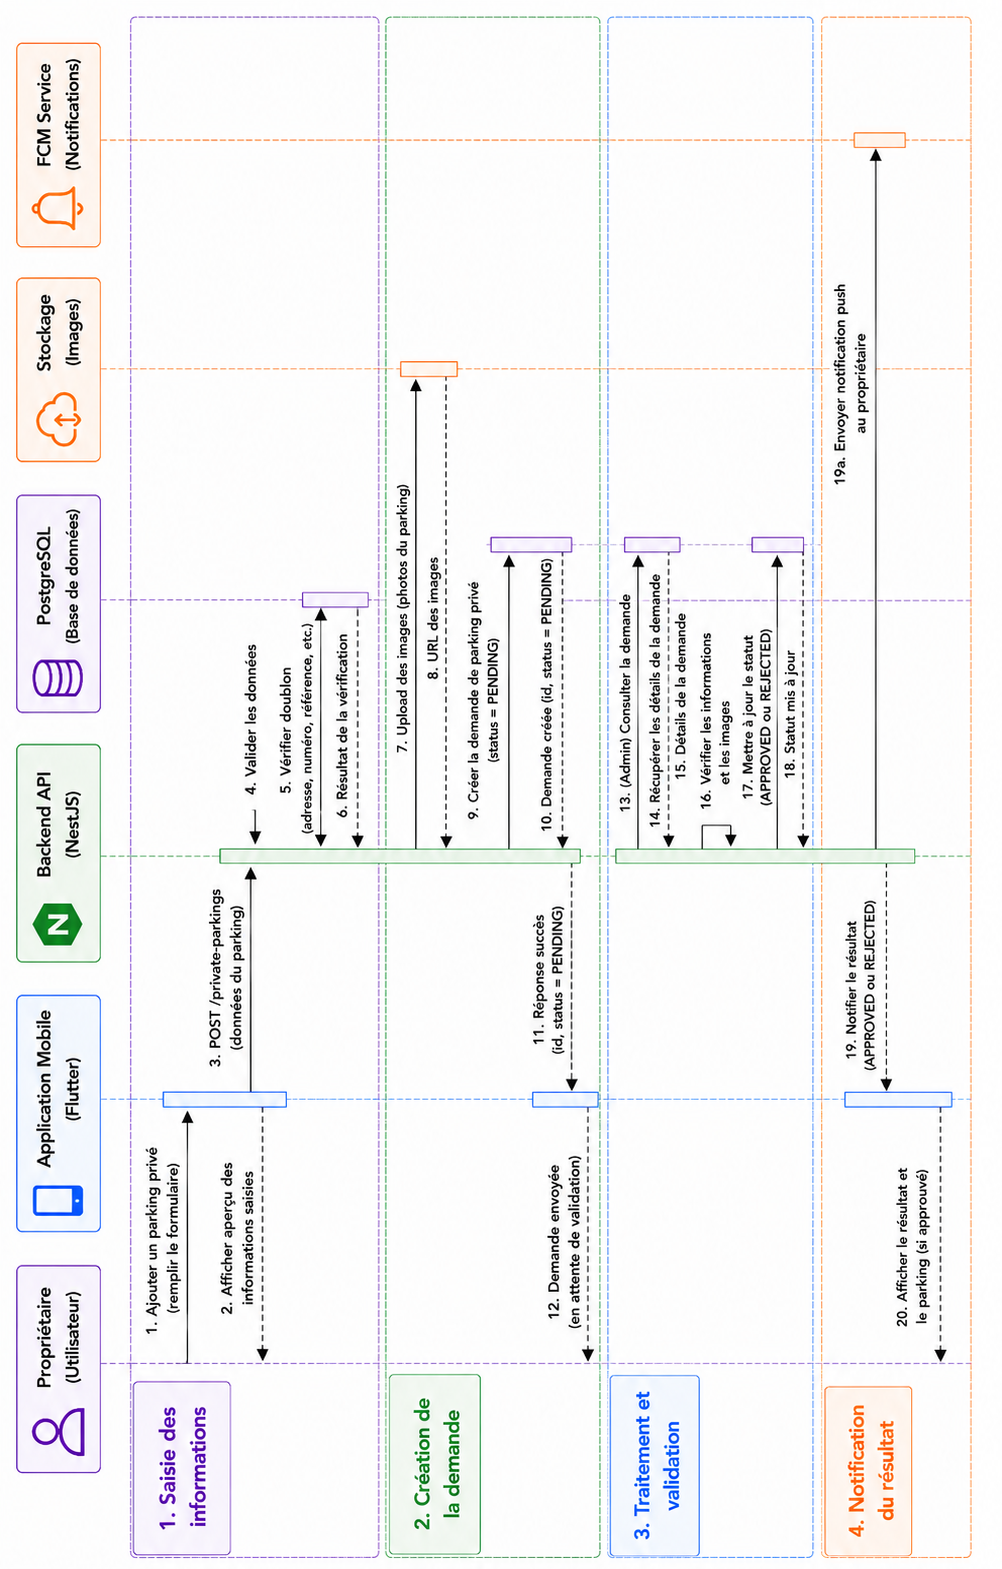
\includegraphics[width=\textwidth]{img/ajout_parking.png}
    \caption{Ajout d'un parking privé}
    \label{fig:sequence_private_parking}
\end{figure}


\subsection{Diagramme de séquence des notifications}

\par Le diagramme de séquence des notifications présente le processus d'envoi d'une notification à un utilisateur de l'application \textbf{TuniPark}. Lorsqu'un événement important se produit, tel que la validation d'un parking privé, la confirmation d'un paiement ou l'activation d'une session de stationnement, le Backend crée une notification et le sauvegarde dans la base de données.

\par Il récupère ensuite les jetons FCM associés à l'utilisateur concerné et transmet le contenu de la notification à \textbf{Firebase Cloud Messaging} \cite{firebase}. Ce service se charge de l'envoyer vers l'appareil mobile de l'utilisateur. La notification reste également disponible dans l'application afin de pouvoir être consultée ultérieurement et marquée comme lue.

\begin{figure}[H]
    \centering
    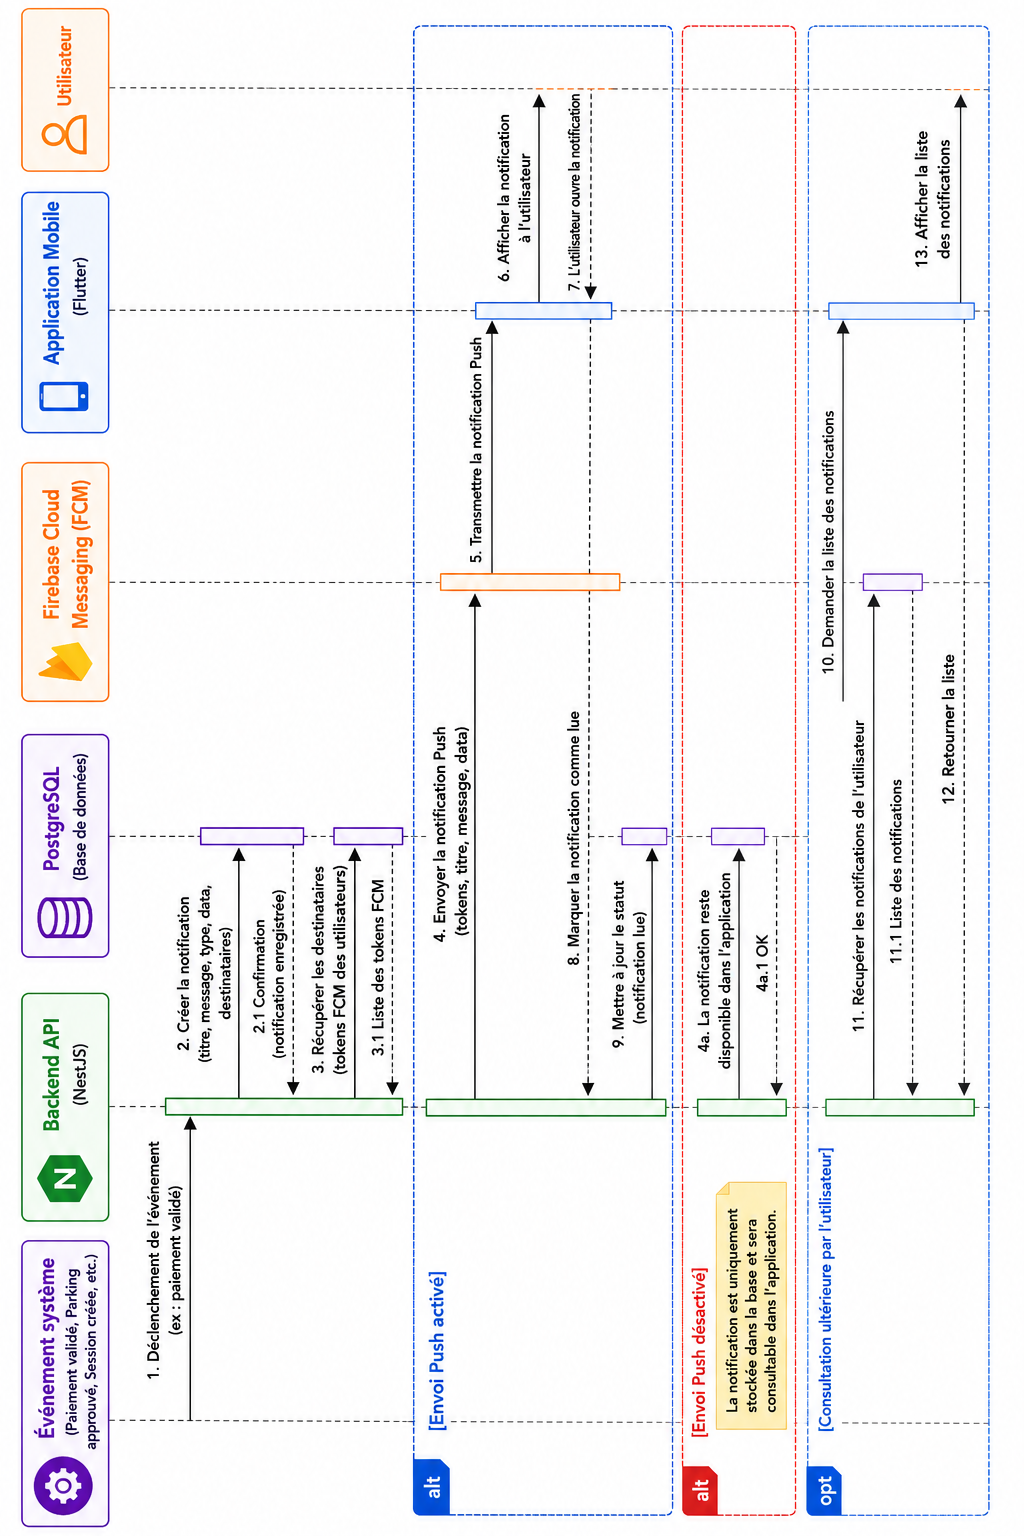
\includegraphics[width=0.95\textwidth]{img/seq_notifications.png}
    \caption{Envoi des notifications}
    \label{fig:sequence_notifications}
\end{figure}

\section{Conclusion}

\par Ce chapitre a présenté la conception et l'architecture de l'application \textbf{TuniPark}. Il a décrit les architectures logique et physique du système, puis les principaux choix techniques retenus pour le développement des différents composants de la solution.

\par Le chapitre a également présenté la conception de la base de données ainsi que les principaux modèles UML utilisés pour représenter le fonctionnement de l'application. Le diagramme de classes a mis en évidence les principales entités du système et leurs relations, Alors que les diagrammes de séquence ont dépeint le déroulement des processus principaux, notamment l'authentification des utilisateurs, la création et le paiement d'une session de stationnement, la recommandation intelligente des parkings, l'ajout d'un parking privé ainsi que l'envoi des notifications.

\par L'ensemble de ces éléments de conception constitue une base robuste pour la phase d'implémentation de l'application. Le chapitre suivant abordera à l'implémentation de TuniPark et présentera les différents modules développés, les interfaces utilisateur ainsi que les principales fonctionnalités mises en œuvre.